\documentclass[11pt]{article}
\usepackage[letterpaper,top=.77in,bottom=.78in,left=.92in,right=.92in]{geometry}
\usepackage{amsmath,amssymb,booktabs,graphicx,xcolor,hyperref,fancyhdr}
\definecolor{teal}{RGB}{0,112,106}\definecolor{ink}{RGB}{26,52,66}\definecolor{muted}{RGB}{62,85,94}
\hypersetup{colorlinks=true,urlcolor=teal,linkcolor=teal,pdftitle={Larger no-three-in-line packings}}
\pagestyle{fancy}\fancyhf{}\renewcommand{\headrulewidth}{0pt}\renewcommand{\footrulewidth}{.35pt}\fancyfoot[L]{\footnotesize\sffamily\color{muted} NO-THREE-IN-LINE \enspace / \enspace COMPUTATIONAL NOTE}\fancyfoot[R]{\footnotesize\sffamily\thepage}
\setlength{\parindent}{0pt}\setlength{\parskip}{6pt}\newcommand{\head}[1]{\par\vspace{4pt}{\Large\sffamily\bfseries\color{ink}#1}\par}\newcommand{\sub}[1]{\par\vspace{3pt}{\large\sffamily\bfseries\color{ink}#1}\par}\newcommand{\eyebrow}[1]{{\small\sffamily\bfseries\color{teal}#1}\par}\newcommand{\file}[1]{\texttt{\detokenize{#1}}}
\newcommand{\diffOne}{163}
\newcommand{\diffTwo}{240}
\newcommand{\diffThree}{192}
\newcommand{\firstAdded}{603}

\begin{document}
\eyebrow{DISCRETE GEOMETRY \quad / \quad RESEARCH FOLLOW-UP \hfill 19 NOVEMBER 2026}
\vspace{3pt}{\LARGE\sffamily\bfseries\color{ink}Larger no-three-in-line packings}\par
A packing here is a set of integer points on $\{0,\ldots,n-1\}^2$ with no three on an ordinary straight line. On three large boards we improve explicit published witnesses by \textbf{\diffOne, \diffTwo{} and \diffThree{} points}. The change is to permit deletions from a classical modular starting set, not just insertions into its gaps. All coordinates and standalone verification code accompany this note.
\sub{How many points fit?}
\begin{center}\small\begin{tabular}{r r r r r}
\toprule Side $n$ & Published witness & This construction & Gain & Points/$n$\\\midrule
16,018 & 24,306 & \textbf{24,469} & +163 & 1.527594\\
32,002 & 48,421 & \textbf{48,661} & +240 & 1.520561\\
64,006 & 96,816 & \textbf{97,008} & +192 & 1.515608\\
131,074 & --- & \textbf{196,650} & --- & 1.500298\\
1,000,018 & --- & \textbf{1,500,030} & --- & 1.500003\\
\bottomrule\end{tabular}
\end{center}
\smallskip
The comparison column is with the three specific witnesses of rStation paper 47, \href{https://rstation.ai/problems/no_three_in_line/papers/47}{\S8}. A dash means no same-board benchmark from that paper. These are lower bounds for the ordinary problem, not unrestricted optima or claims of worldwide priority. The much larger grids test feasibility, not a better limiting density.
\begin{center}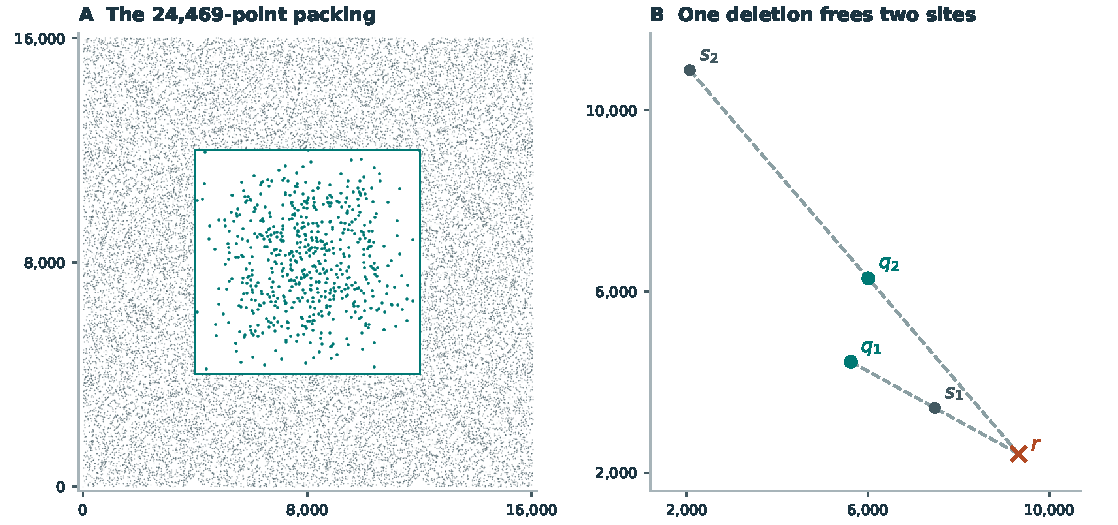
\includegraphics[width=.94\linewidth]{exchange-figure.pdf}\end{center}
{\small\textbf{A.} Retained frame sites are grey; the \firstAdded{} additions are teal. \textbf{B.} An actual exchange starting from the published 24,306-set. Each proposed point $q_i$ has exactly one obstructing pair, $\{r,s_i\}$. Remove $r=(9327,2418)$ and both $q_1=(5625,4448)$ and $q_2=(6009,6289)$ can be added together. The resulting gain of one does not require moving any other point.}
\sub{The million-wide case, in six coordinates}
At $p=500009$, keep the whole frame defined on page 2 and add the points below. They give $1,500,030$ points, three more than $3n/2$:
\[
\begin{array}{ccc}
(500009,498618)&(500009,499724)&(501011,499220)\\
(501819,500429)&(499007,500797)&(498199,499588).
\end{array}
\]

\newpage
\eyebrow{01 \quad / \quad THE MODULAR CONSTRUCTION}
\head{What if the frame cannot be changed?}
For an odd prime $p$ put $h=(p-1)/2$, $J=\{h+1,\ldots,h+p\}$ and $n=2p$. We use the same translated Hall--Jackson--Sudbery--Wild frame as the benchmark:
\[
 S_p=\{(x,y)\in\{0,\ldots,2p-1\}^2:x(y-h)\equiv1\pmod p\}\setminus J^2.
\]
There are $p-1$ possible nonzero $x$-residues, each with four lifts, one excluded. Thus $|S_p|=3(p-1)$. The sets we construct are $(S_p\setminus R)\cup A$. The numbers in the next table count sites that can be added \emph{without removing any part of $S_p$}, over the whole board, not only inside $J^2$.
\begin{center}\small\begin{tabular}{r r r r r}
\toprule Side & Individually legal & Simultaneously legal$^{*}$ & Frozen total$^{*}$ & With deletions\\\midrule
16,018 & 388 & 284 & 24,308 & 24,469\\
32,002 & 614 & 424 & 48,424 & 48,661\\
\bottomrule\end{tabular}
\end{center}
{\footnotesize $^{*}$Exact subject to retaining $S_p$. ``Individually legal'' means a site lies on no line through two frame points. The last column drops that retention constraint and gives lower bounds only.}\par
\textbf{Certificate of optimality.} First discard filled rows and columns (two frame points already). For every pair of frame points, walk its entire lattice line in primitive integer steps and strike out the visited cells. The unoccupied survivors are the complete lists of 388 and 614 individually legal sites. The released sets of 284 and 424 additions verify directly, giving the lower bounds.

For the upper bounds, use disjoint groups of surviving sites. On side 16,018 there are 95 pairs that cannot coexist: in each, the line through the pair contains a retained frame point. There are also five collinear triples and one collinear six-set. These force at least $95+5+4=104$ omissions, leaving at most $388-104=284$. On side 32,002 there are 166 incompatible pairs, four groups of three in which every pair is incompatible, and two collinear ten-sets. They force $166+4\cdot2+2\cdot8=190$ omissions, leaving $614-190=424$. The certificates list every site and blocking frame point; the verification does not require a solver.

\sub{How the exchanges were found}
We searched for sites lying on few lines through pairs of starting points. For a site blocked by just one surviving pair, either endpoint is a possible deletion. Grouping sites by a shared endpoint identifies exchanges of one old point for two or more new ones. At each step we also test lines determined by two new sites: individually permissible additions need not coexist. Randomized ordering gave different compatible exchanges. The search is heuristic; the checks below are not.
\sub{Why the verification covers every triple}
A primitive integer line remains a genuine line modulo $p$. It meets $x(y-h)=1$ in at most two residues (substitution gives a quadratic, or a single root for a vertical line). Any collinear triple of retained frame points would therefore include two congruent points. In a box of side $2p$ their direction is horizontal, vertical or of slope $\pm1$. The verifier counts every retained point on each of those four line families and rejects any count greater than two.

For each $q\in A$, the checker reduces $v-q$, for every other final point $v$, to an unoriented primitive direction by dividing by the gcd and fixing the sign. Two directions coincide exactly when they form a collinear triple through $q$. Thus triples involving additions, including those involving three additions, are checked as well. No floating-point tolerance or trust in the discovery program is needed.
\newpage
\eyebrow{02 \quad / \quad DENSITY AND SYMMETRY}
\head{Two boards just above $1.8n$}
Start with the 360-point configuration \file{sets/n200_c.txt} from \href{https://rstation.ai/problems/no_three_in_line/papers/22}{kiro\_conic, paper 22, v4}, converting its coordinates to start at zero. No deletions are needed. In the original coordinate system, the only individually legal additions in the surrounding $204\times204$ window are
\[
 (-1,145),\quad (145,200),\quad (200,54),\quad (54,-1).
\]
For side 201 take the first two and translate by $(1,0)$: \textbf{362 points}, or $1.800995n$. For side 202 take all four and translate by $(1,1)$: \textbf{364 points}, or $1.801980n$. The four sites form a quarter-turn orbit. Since the seed already spans 200 rows and 200 columns, no three of the four fit together at side 201. These are the best extensions \emph{retaining this whole seed up to translation}, not upper bounds on other packings. Direct integer tests checked all 7,840,920 and 7,971,964 respective triples.
\sub{Full square symmetry: exact values at 67 and 69}
Write $F(n)$ for the optimum under all eight symmetries. On an odd board $n=2m+1$ a noncentral orbit uses two magnitudes and supplies eight sites, or one magnitude and supplies four (axis or diagonal). Separate orbits cannot share a positive magnitude: one row would then contain more than two sites. The centre cannot coexist with an opposite pair. Hence the candidate sizes above one are $4(m-k)$ for $k$ unused magnitudes.
\begin{center}\small\begin{tabular}{r r r r r}\toprule
Side & Points tested & Sets found & Orbit-counter nodes & Line-counter nodes\\\midrule
67 &132&0&56,889,403&56,889,403\\
67 &128&1&695,639,247&719,417,016\\
69 &136&0&106,477,824&106,477,824\\
69 &132&0&1,331,533,733&1,375,772,064\\\bottomrule
\end{tabular}\end{center}
Thus $F(67)=128$, with a unique maximizing set. Centre that same set on the 69-board to attain 128 again. The two empty tiers above it give $F(69)=128$ \emph{without} needing a count at 128; its multiplicity at 69 is not reported. The two counters generate conflicts independently, one from directions through orbit points and one from actual grid lines.
\sub{What did not work at 75, 77 and 79}
For five neighbouring published $2m$-point packings ($m=74,74,76,76,78$), insert an empty row and column in all possible positions and put a point at their intersection. All \textbf{29,349} trials had a collinear triple; the respective minimum numbers of triples were $6,6,7,7,6$. This excludes only this transformation of these five seeds. We found no 149-, 153- or 157-point witness on those three boards.

{\footnotesize\textbf{Sources and reproduction.} Classical frame: \href{https://doi.org/10.1016/0097-3165(75)90043-6}{Hall, Jackson, Sudbery and Wild (1975)}. Benchmark and medium-board coordinates: rStation papers 47 and 22 as linked above. Frontier seeds: \href{https://wwwhomes.uni-bielefeld.de/achim/no3in/readme.html}{Flammenkamp's catalogue}. The accompanying archive records exact input versions, checksums, complete coordinates, code and verification transcripts; start with \file{README.md}.}
\end{document}
